\section{Question 4}
\paragraph{(a)} Considering transfer function
\begin{equation}
G = \frac{10}{s^3 + 10s^2 + 16s},
\end{equation}
\noindent then, state-state representation in canonical form is
\begin{equation*}
A_c =
\begin{bmatrix}
-10 & - 16 	& 0 \\
1   &  	0	& 0 \\
0 	&	1 	& 0 	
\end{bmatrix},
B_c =
\begin{bmatrix}
1 \\ 0 \\ 0
\end{bmatrix},
C_c = 
\begin{bmatrix}
0 	& 	0 	& 	10
\end{bmatrix},
D_c =
\begin{bmatrix}
0
\end{bmatrix},
\end{equation*}
and state-state representation in observable form is
\begin{equation*}
A_o =
\begin{bmatrix}
-10 	&   1 	& 0 \\
-16 	& 	0	& 1 \\
  0 	&	0 	& 0 	
\end{bmatrix},
B_o =
\begin{bmatrix}
0 \\ 0 \\ 10
\end{bmatrix},
C_o = 
\begin{bmatrix}
1 	& 	0 	& 	0
\end{bmatrix},
D_o =
\begin{bmatrix}
0
\end{bmatrix}.
\end{equation*}

\paragraph{(b)} The controller gains can are $k_c=\begin{bmatrix}
-47.1 & 5.84 & -0.66
\end{bmatrix}$ and observer gains are $k_o = \begin{bmatrix}
0.25 & 59.5 & 212
\end{bmatrix}$.


\paragraph{(c)} Figure \ref{fig:plot_equation_3d} shows the performance of close loop system with controller and observer when initial condition is $\mathbf{x}=\begin{bmatrix}
1 & 0 & 0
\end{bmatrix}$$^T$ 

\begin{figure}
\centering
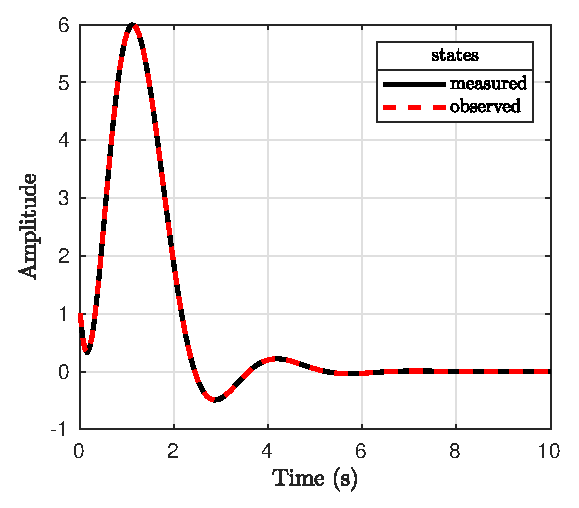
\includegraphics{images/plot_question_3d.eps}
\caption{Close loop system with controller poles $s=-1.4,s=-1\pm2.15i$ and observer poles $s=-4.25,s=-3\pm6.4i$.}
\label{fig:plot_equation_3d}
\end{figure}